\section{Einleitung}
\subsection{Automatische Musiktranksription}
Musik war schon immer ein zentraler Bestandteil unserer Gesellschaft.
Während früher musikalische Werke meist mündlich überliefert wurden,
entwickelte sich während des Mittelalters die Notenschrift, welche wir auch heutzutage noch nutzen.
Diese Notenschrift ermöglichte es, Musikstücke einfacher zu erlernen und Musik einem breiteren Publikum zugänglich zu machen.
Durch die Digitalisierung erhielten \("\)Digital Audio Workstations\("\) zunehmend Einzug in die Musikproduktion,
wodurch Notenblätter irrelevanter wurden und somit weniger Musikstücke in Notenschrift übersetzt wurden.

Ungefähr gleichzeitig begann zudem die Forschung an AMT-Systemen (Automatic Music Transcription).
AMT ist ein Prozess, zur automatischen transkription von Audiospuren.
Als Input wird ein Audiosignal gegeben, welches durch verschiedene Prozesse umgewandelt wird.
Diese Prozesse analysieren die Eigenschaften der Noten, zum Beispiel die Frequenz, Lautstärke und vieles mehr.
Dadurch entsteht als Output eine MIDI-Datei, ein Notenblatt oder andere Daten,
die das gegebene Musikstück in Schriftform darstellen.

\subsection{Herausforderungen und Hindernisse}
Anstatt durch sein Gehör selber diese Musikstücke in Notenschrift zu übertragen,
würde ein AMT-System diese Aufgabe für einen übernehmen.
Dieses Ziel ist jedoch schwer zu erreichen,
da Musik mehrdimensional ist durch zum Beispiel Zeit, Tonhöhe und Polyphonie.
Vor allem bei polyphonen Musikstücken haben herkömmliche Algorithmen häufig Schwierigkeiten.
In diesen Fällen müssen sie nämlich mehrere verschiedene Stimmen gleichzeitig analysieren und
im späteren auch die jeweiligen Töne voneinander differenzieren und eindeutig einem Instrument zuordnen.
Ein weiteres Problem ist die Individualität jedes Musikstückes.
In realen Aufnahmen können leichtes Rauschen,
kleine Spielfehler oder stilistische Mittel wie Vibrato auftreten,
die je nach Interpreten unterschiedlich klingen.
Zudem sind die meisten AMT-Modelle auf westliche Tonleiter trainiert.
Dies kann zu Problemen führen, wenn zum Beispiel
arabische oder indische Musikstücke transkribiert werden sollen.

In folgender Tabelle sind einige Regionen aufgelistet und deren Tonleiter, die diese benutzen.
Die Tabelle ist nicht vollständig, auf der Welt gibt es noch viele weitere Regionen, welche auch ihre ganz eigenen Tonleiter nutzen.
\begin{table}[H]
\centering
\begin{tabular}{|l|p{10cm}|}
\hline
\textbf{Region} & \textbf{Typische Skalen} \\ \hline
Europa & Dur, Moll, Kirchentonarten, Pentatonik \\
\hline
Arabische Welt & Maqām Rast, Maqām Bayati, Maqām Hijaz, Maqām Kurd, Maqām Nahawand \\
\hline
Türkei & Hicaz, Nihavent, Hüseyni, Segah, Uşşak \\
\hline
Persien / Iran & Shur, Mahur, Segah, Homayun, Nava \\
\hline
Indien & Rāga Yaman, Bhairav, Todi, Kafi, Bhupali \\
\hline
China & Gong, Shang, Jue, Zhi, Yu \\
\hline
Japan & Hirajoshi, In-sen, Yo, Kumoi \\
\hline
Indonesien & Sléndro, Pélog \\
\hline
Afrika & Pentatonik, Hexatonik, Balafon-Skalen \\
\hline
\end{tabular}
\caption{Übersicht typischer Skalen verschiedener Weltregionen}
\end{table}

\subsection{AMT und Künstliche Intelligenz}
Um diese musikalische Vielfalt zu bewältigen, wird heutzutage künstliche Intelligenz und Machine Learning eingesetzt.
Im Gegensatz zu Algorithmen ist KI flexibler und kann sich dadurch besser
auf kleine Abweichungen in Musikstücken einstellen.
Ein Audiosignal kann entweder im Studio produziert oder im Alltag aufgenommen werden.
Alltag aufgenommene Signale werden, in dieser Arbeit, als reale Audiosignale bezeichnet.
Reale Audiosignale besitzen immer eine gewisse Menge an Rauschen.
Das kann bei der automatischen Musiktranskription für schwierigkeiten sorgen,
da Algorithmen diese als zusätzliche Noten ansehen oder richtige Noten dadurch nicht erkennen könnten.
KIs können sich besser an die fehlerhaften Geräusche von Rauschen anpassen,
da neuronale Netzwerke mit genau diesen unperfekten Audiosignalen trainiert werden können.
Somit können AMT-Systeme besser angepasst werden für einen realistischen Alltagsgebrauch.

Auch die Mehrdimensionalität von Musik kann KI deutlich besser bewältigen als Algorithmen.
Neuronale Netze besitzen eine mehrdimensionale Struktur, die es ihnen ermöglicht,
verschiedene Muster, Stimmen und Eigenschaften zu erlernen.
\cite{graves2007multi}
Auf der anderen Seite müssen klassische Algorithmen diese verschiedenen Dimensionen
explizit modellieren und sind nicht in der Lage, Muster selbstständig zu erkennen.
Sie folgen nur den fest einprogrammierten Anweisungen und sind somit nicht anpassungsfähig.

In der automatischen Musiktranskription wird das Input Audiosignal immer zunächst in ein Spektrogramm umgewandelt.
Spektrogramme zeigen den zeitlichen Verlauf des Frequenzspektrums eines Audiosignals.
Es gibt verschiedene Arten von Spektrogrammen.
Zwei Spektrogrammtypen, die häufig genutzt werden, sind CQT-Spektrogramme und Log-Mel-Spektrogramme.
CQT steht für Constant-Q Transform und in diesem Spektrogramm werden die Frequenzachsen logarithmisch aufgelöst.
Zudem bleibt der Q-Faktor konstant, dieser beschreibt das Verhältnis von Frequenz zu Brandbreite.
Das Log-Mel-Spektrogramm wird zunächst mit einer Short-Time Fourier Transform (STFT) gebildet.
STFT ist eine Methode, um ein Signal als ein Frequenzspektrum darzustellen.
Anschließend wird die lineare Frequenzachse auf eine Mel-Skala projiziert.
Das menschliche Gehör kann zum Beispiel 200--400Hz feiner als 5000--5200Hz wahrnehmen.
Die Mel-Skala sorgt dafür, das sich das Spektrogramm dem menschlichen Gehör anpasst.
Insgesamt ist ein CQT-Spektrogramm besser für die automatische Musiktranskription,
da in diesem die Töne feiner unterschieden werden können.
Jedoch werden in neueren KI-Modellen zum großteil Log-Mel-Spektrogramme genutzt.
Diese sind robuster und funktionieren, vor allem in Transformer-basierte KI-Modellen, zuverlässiger.

Im Folgenden sind vier verschiedene Spektrogramme zu sehen,
welche alle auf den identischen Ausschnitt aus Bachs WTK I, Nr.5 \cite{bach_wtk1_nr5} basieren.
Oben links ist ein normales lineares Spektrogramm zu sehen,
welches ausschließlich auf dem STFT basiert und eine lineare Frequenzskala besitzt.
Rechts daneben ist ein Log-Spektrogramm,
bei dem die Amplitudenwerte des STFT logarithmisch in Dezibel skaliert wurden,
wodurch der Dynamikumfang im niedrigen Amplitudenbereich erhöht wird.
Das \("\)MelSpec\("\) steht für Log-Mel-Spektrogramm und unten rechts wird ein CQT-Spektrogramm angezeigt.
\begin{figure}[H]
    \centering
    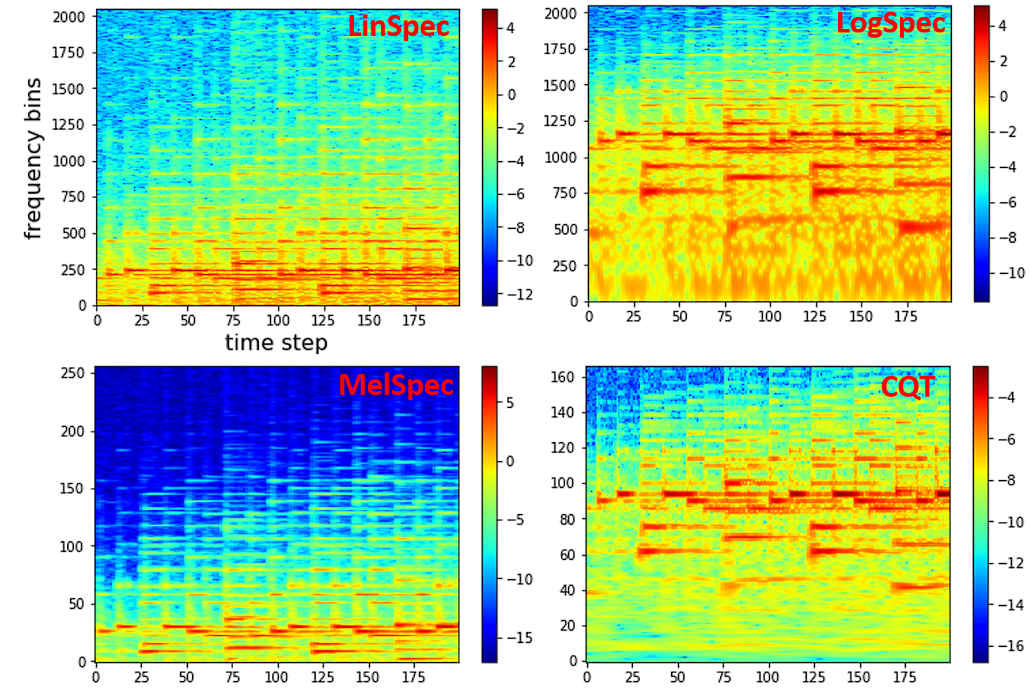
\includegraphics[width=1\textwidth]{Graphics/different_spectrograms}
    \caption[Vergleich 4 Spektrogramme]{Vergleich von vier Spektrogrammen basierend auf \cite{cheuk2020impact}.}
    \label{fig:different_specs}
\end{figure}

Es gibt verschiedene KI-Modelle, welche für AMT-Systeme in Frage kommen.
In diesem Abschnitt werden die am weitesten verbreiteten KI-Modelle aufgegriffen.
Weitere potenzielle KI-Modelle und der heutige
\("\)State of the Art\("\) werden im Abschnitt-\titleref{sec:ki_integration} ausführlich erläutert.
Die meisten AMT-Systeme nutzen Recurrent Neural Networks (RNN) und Convolutional Neural Networks (CNN).
\cite{Boeck2012}
Diese Module bilden keine eigenständigen Systeme, sondern lassen sich flexibel innerhalb eines Systems kombinieren.
Da es keine objektiv richtigen oder falschen Notenfolgen gibt, ist der Einsatz von Supervised Learning am effizientesten.
Dementsprechend ist es notwendig ein zuverlässiges und großes Datenset aus Audiodateien und deren zugehörigen MIDI-Dateien zu besitzen.

CNNs können gut räumliche Strukturen erkennen.
Das ist sehr hilfreich bei der Analyse von Spektrogrammen.
Da das Input Audiosignal in ein Spektrogramm umgewandelt wird,
kann das CNN diese bildliche Darstellung analysieren.
Durch die Analyse von dem Spektrogramm können gewisse Frequenzmuster erkannt werden,
die darauffolgend einem bestimmten Instrument zugeordnet werden können.
Das ist vor allem hilfreich dabei verschiedene Stimmen der jeweiligen Instrumente voneinander zu differenzieren.
\cite{han2016deep}

RNNs hingegen spezialisieren sich darauf, mithilfe eines Gedächtnis, zeitliche Abläufe zu verstehen.
In Musikstücken werden zahlreiche Noten hintereinander gespielt, welche harmonisch aufeinander aufbauen.
Das RNN verarbeitet die jeweiligen Sequenzen und merkt sich die Informationen der schon gespielten Noten,
um die darauffolgenden Noten besser einordnen zu können.
So lässt sich die harmonische Struktur des Musikstückes analysieren.
Auch der Rhythmus und vorhandene Vorzeichen lassen sich dadurch interpretieren.
\cite{Boeck2012}

In den meisten AMT-Systemen werden RNNs und CNNs kombiniert.
Zunächst verarbeitet das CNN das Spektrogramm und extrahiert dabei musikalische Merkmale.
Darauf folgend verarbeitet das RNN diese Merkmale und bildet konkrete Noten mit deren einzelnen Eigenschaften.
\begin{enumerate}
    \item \textbf{CNN:} Extrahiert folgende Merkmale aus dem Spektrogramm:
    \begin{itemize}
        \item Frequenzverteilungen und spektrale Muster
        \item Tonhöhenlage und damit verbundene Obertöne
        \item Klangfarbe einzelner Instrumente
        \item Energieverteilung, unter anderem zur Erkennung von Toneinsätzen
        \item Harmonische Strukturen wie Akkordfolgen
    \end{itemize}

    \item \textbf{RNN:} Verarbeitet auf Basis dieser Merkmale die zeitliche Abfolge und erkennt dabei folgende Eigenschaften:
    \begin{itemize}
        \item Reihenfolge und Übergänge musikalischer Ereignisse
        \item Beginn und Ende einzelner Töne zur Bestimmung der Notendauer
        \item Rhythmische Muster und zeitliche Gruppierungen
        \item Musikalische Phrasen mit zusammenhängender Struktur
        \item Wiederholungen, Themen oder längere Abhängigkeiten im Verlauf
    \end{itemize}

    \item \textbf{Output:} Gibt das transkribierte Musikstück in strukturierter Form aus:
    \begin{itemize}
        \item Als MIDI-Datei mit exakten Noteninformationen
    \end{itemize}
\end{enumerate}
Nachdem die KI-Modelle die Daten verarbeitet haben, kann die erhaltene MIDI-Datei mit einem externen Programm
zu standardisierten Musiknoten transkribiert werden.

\subsection{Anwendungsfelder und Vorteile}\label{subsec:praktisch}
AMT kann auch häufig bei anderen Problemen helfen
oder in zahlreichen Bereichen Quality-of-Life-Changes bringen.
Zum einen kann der Musikunterricht spannender und interaktiver gestaltet werden.
Es würde eine breitere Auswahl von Musikstücken geben, die den Schülern angeboten werden können,
wodurch diese durch individuell angepasste Musikstücke mehr Spaß und Ehrgeiz beim Lernen entwickeln.
Zudem können die gespielten Musikstücke der Schüler während des spielens transkribiert werden,
wodurch frühzeitig erkannt wird, wo der jeweilige Schüler noch Verbesserungsmöglichkeiten aufweist und Feedback erhalten muss.
Grundsätzlich können deutlich mehr Musikstücke transkribiert werden,
wodurch sich große Archive aufbauen lassen.
Ein größeres Interesse an Musik wird geweckt, da Musikstücke von beliebten Serien, Filmen oder Spielen
leichter für deren Musikbegeisterte Zielgruppe zugänglich sind.
Alleine dadurch, dass KI-Modelle Musikstücke besser verstehen,
können darauf aufbauend weitere Tools für die Musikproduktion entwickelt werden.
Auch andere Anwendungsfelder von künstlicher Intelligenz würden dadurch profitieren.
KI-generierte Musik würde verbessert werden, da die KI selber ein besseres Verständnis der Musik entwickelt.
Audiobasierte Suchmaschinen könnten gewünschte Musikstücke oder bestimmte Videos präziser finden.

\subsection{Motivation, Zielsetzung und Ablauf}
Künstliche Intelligenz ist eins der momentan aktivsten Forschungsfelder.
Durch KIs wurden und werden noch viele grundlegende Probleme
und Algorithmen komplett umstrukturiert, verworfen oder gelöst.
Ein Forschungsgebiet, das unter anderem auch sehr stark durch die Einführung von KI profitiert hat,
ist die automatische Musiktranskription.
Während früher noch Modelle und Algorithmen genutzt worden, um AMT-Systeme umzusetzen,
werden jetzt überwiegen verschiedene KI-Modelle genutzt,
um unter anderem Spektrogramme zu analysieren und um den Aufbau des Musikstückes zu identifizieren.

Durch die integration von KI in AMT-Systemen rückt die vorstellung von AMT-Systemen,
welche im alltag genutzt werden auch immer näher.
Sobald das erste AMT-System praxisgeeignet ist, werden sich, wie im Abschnitt-\titlerefN{subsec:praktisch} angeschnitten,
viele neue Einsatzmöglichkeiten ereignen.
Dadurch werden andere Forschungsgebiete gefördert, momentane Aufgaben vereinfacht und das Bildungswesen verbessert.

Deshalb wird der Schwerpunkt dieser wissenschaftlichen Vertiefung darin liegen,
auf die Funktion von KI-Modellen in AMT-Systemen.
Diese Analyse wird sich aus drei Teilen zusammenfügen.
Zunächst werden die heutigen Schwachstellen moderner AMT-Systeme aufgelistet.
Als Nächstes werden die KI-Systeme beschrieben,
welche grundlegend in AMT-Systemen genutzt werden und welche Vorteile diese mit sich bringen.
Zuletzt werden zwei neu zeitige AMT-Systeme vorgestellt,
welche beide eine starke Auswirkung auf dieses Forschungsgebiet haben.

Um das Thema automatische Musiktranskription zu vervollständigen,
wird im nächsten Kapitel zunächst auf die Geschichte von AMT-Systemen eingegangen,
und wie frühere AMT-Systeme funktioniert haben und aussahen.